\documentclass{article}

% Language setting
% Replace `english' with e.g. `spanish' to change the document language
\usepackage[english]{babel}

% Set page size and margins
% Replace `letterpaper' with `a4paper' for UK/EU standard size
\usepackage[letterpaper,top=2cm,bottom=2cm,left=3cm,right=3cm,marginparwidth=1.75cm]{geometry}

\renewcommand{\familydefault}{\rmdefault}

% Useful packages
\usepackage{amsmath}
\usepackage{graphicx}
\usepackage[colorlinks=true, allcolors=blue]{hyperref}

\title{Eurovision survey}
\author{Zvereva Arina}

\begin{document}
\maketitle

\section{Introduction}
This paper is based on \href{https://github.com/rfordatascience/tidytuesday/blob/master/data/2022/2022-05-17/eurovision.csv}{Eurovision dataset} which you can find here. We will look into whether running order of the artist has any impact on the resulting score or rank. We will use a scatter plot and a heat map to help us demonstrate the results. 

\section{Graphs}

\subsection{Scatterplot}

To visualise the running order and the rank of the artist we used a scatterplot. As can be seen there is no strong correlation between these two variables. To support our claim, we provide Figure \ref{fig:scatter} notation .

\subsection{Heatmap}

Provide a heatmap where the X axis is the year of the event, Y axis is the country, and cell colour/hue the country rank at the given year.

Here we have a heatmap which shows distribution between the year of the event (the X axis) and the country (the Y axis), cell colour is responsible here for the country rank at the given year. The lighter the colour, the bigger the rank. See Figure \ref{fig:heatmap} to view the results. 


\begin{figure}
\centering
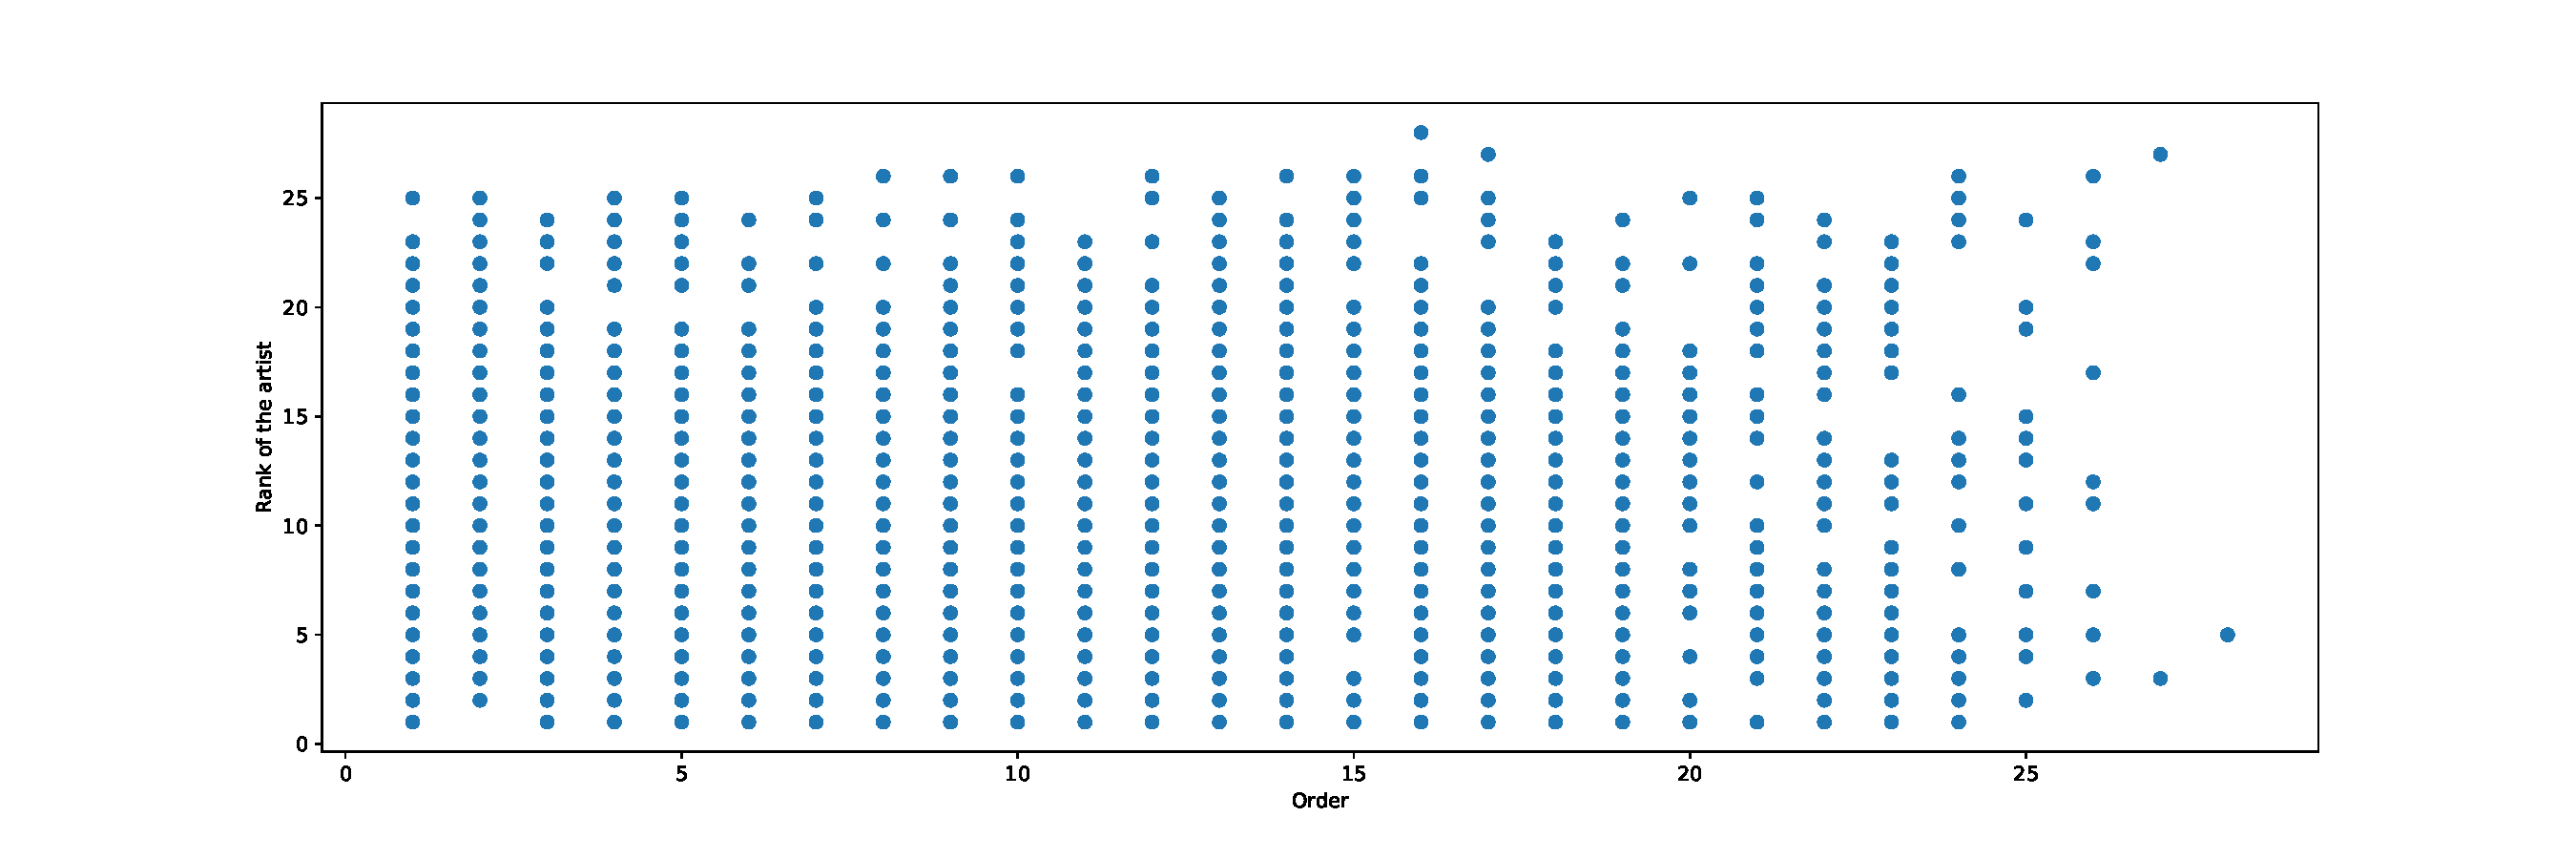
\includegraphics[width=1\textwidth]{figscatter.pdf}
\caption{\label{fig:scatter} Our scatterplot.}    
\end{figure}

\begin{figure}
\centering
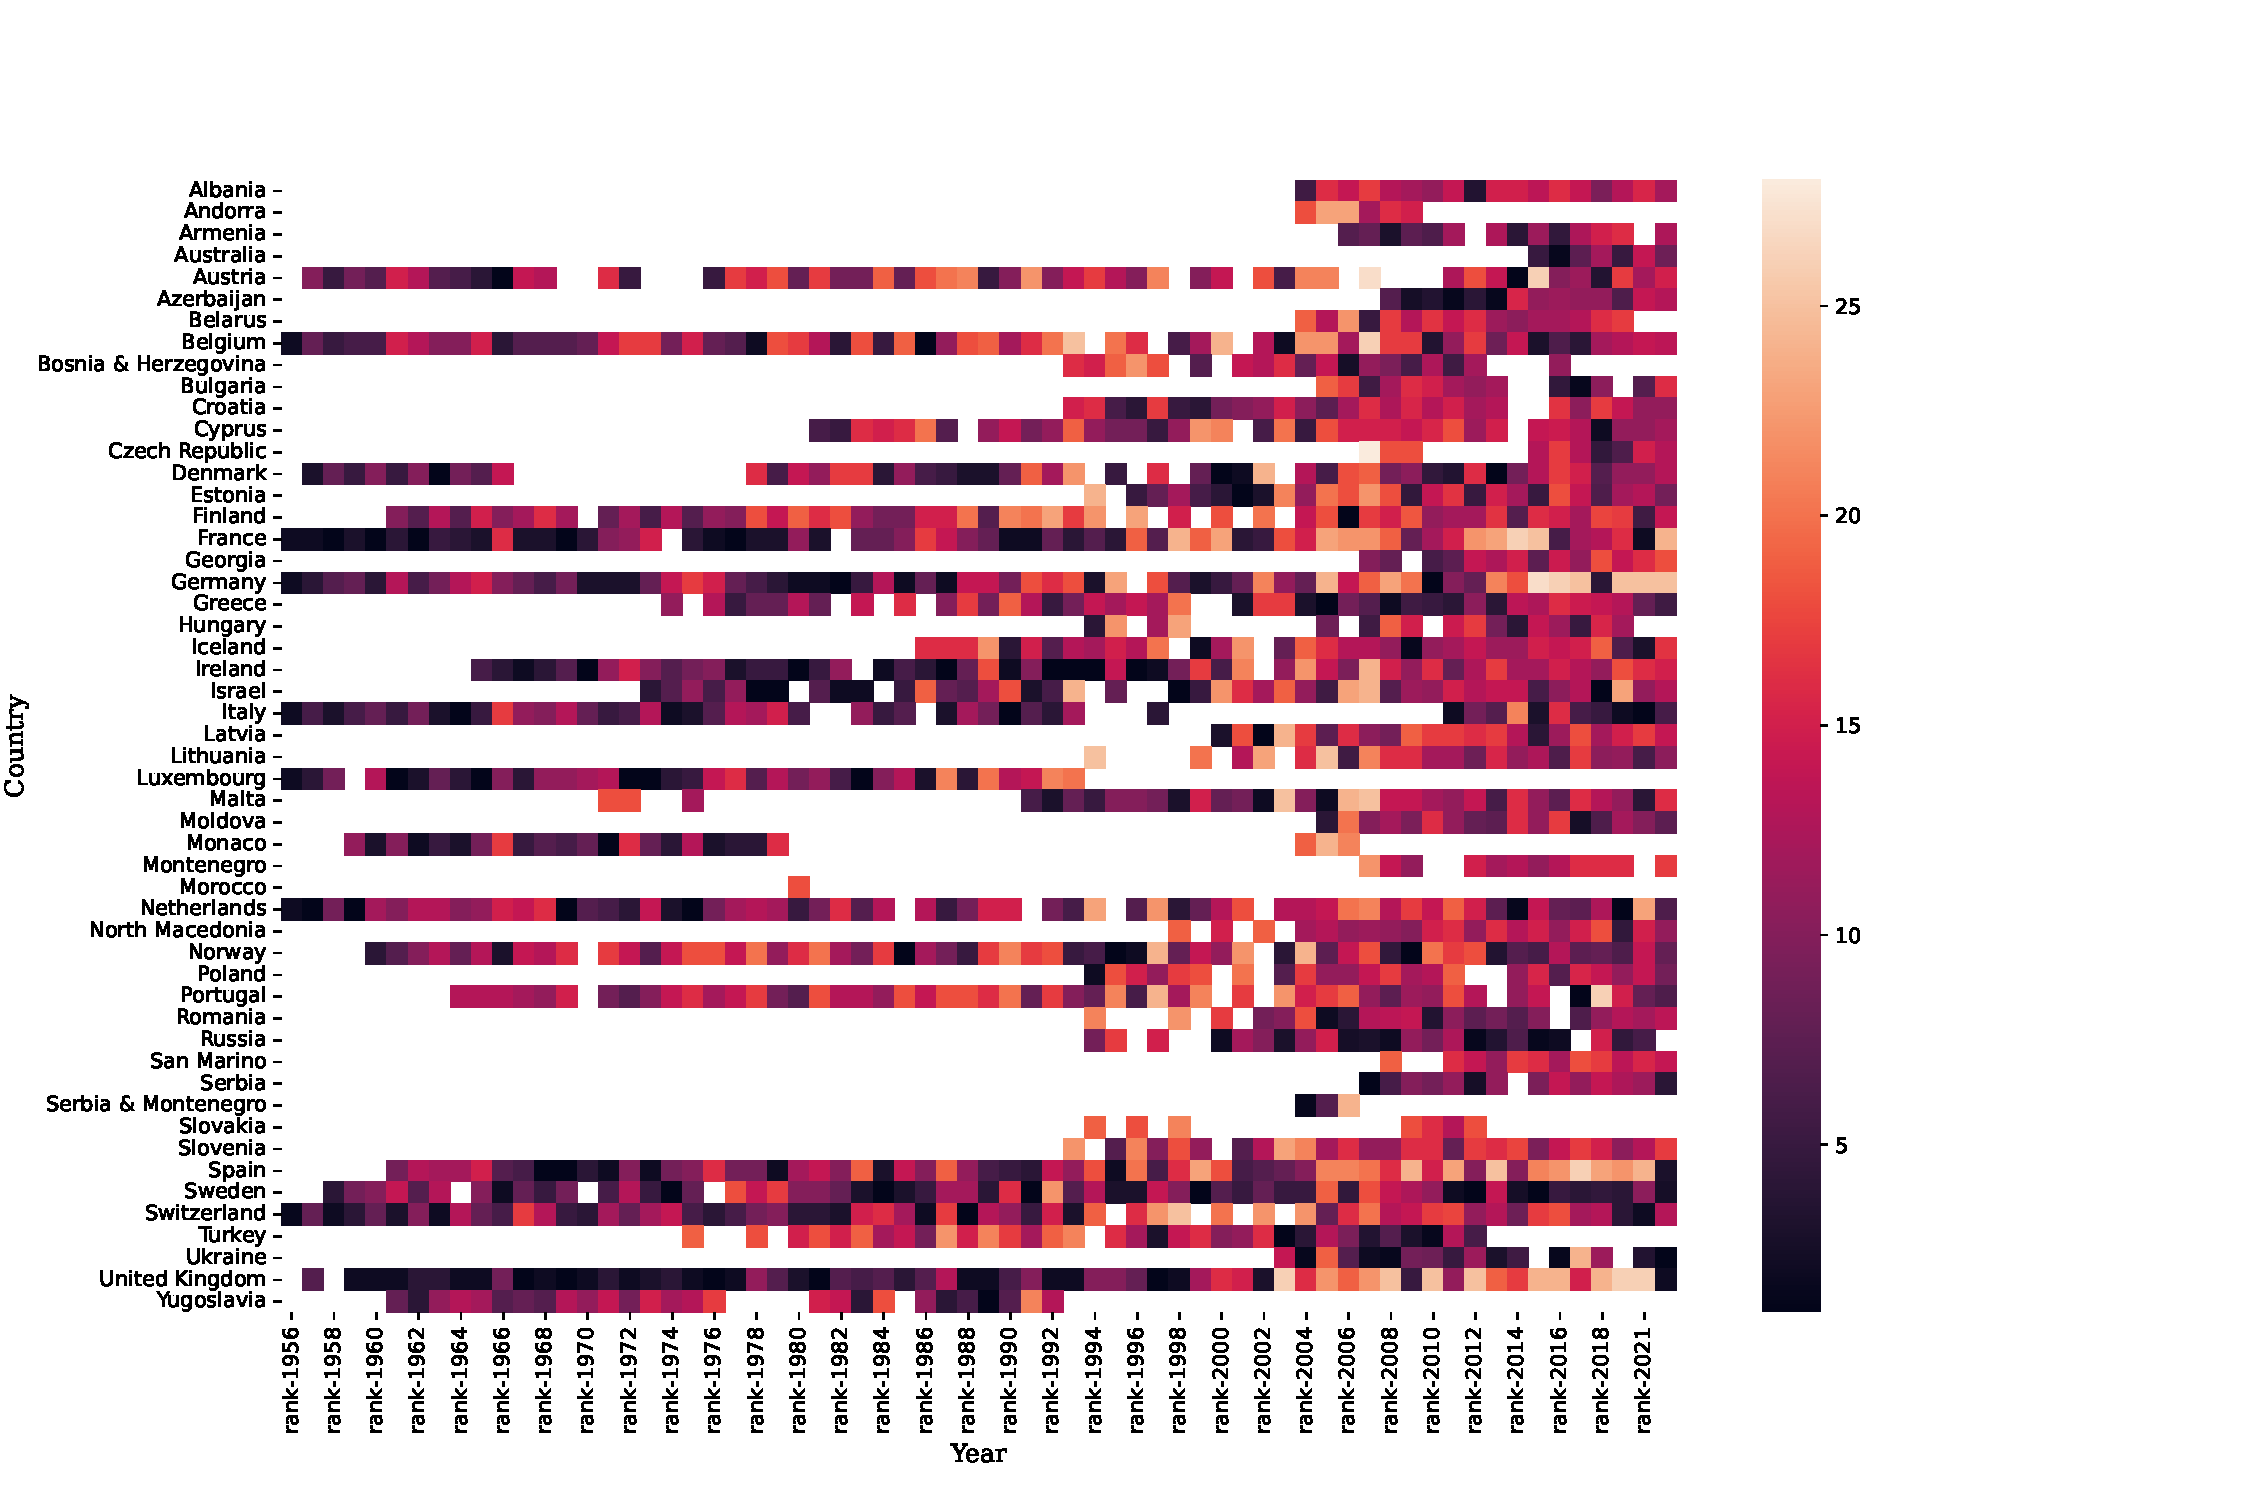
\includegraphics[width=1\textwidth] {figheatmap.pdf}
\caption{\label{fig:heatmap} Our heatmap}
\end{figure}

\section{Recommendations}

For further research we recommend looking into \cite{geslers}. 
\clearpage
\bibliographystyle{alpha}
\bibliography{cite}

\end{document}